\chapter{Material e Métodos}]

\label{chap:Material e Métodos}

\section{Sujeito}
O objetivo desse projeto é construir um jogo da memória executável pelo navegador, podendo ser acessado ao entrar em um site na web, com modos de jogo singleplayer, onde o jogador tentará resolver os desafios sozinho e receber o tempo que demorou para concluir seu desafio ou, jogar no modo multiplayer onde outros jogadores compartilharão o mesmo desafio gerado e disputarão para saber quem consegue finalizar no menor tempo possível. Além disso, e necessário ser possível mudança de dificuldade ao ampliar o numero de itens a serem memorizados.

Porém o aspecto principal desse jogo e o desafio a ser superado é que sua interface e seu todos os aspectos de interface humano-maquina sejam construídos de forma a permitir que pessoas cegas, portadoras de deficiência visual graves possam jogar, e ser competitivas, independente de suas deficiências utilizando de interfaces acessíveis e inteligentes, que possam se adaptar a deficiências do jogador. Nesse sentido, o desenvolvimento de uma experiência e um tecnologia de interface homem-maquina que consiga superar esse desafio é o maio enfoque deste estudo.

Dessa forma as definições dos requisitos em formatos de histórias de usuário seguem da seguinte maneira.

\begin{alineascomnumero}
  \item Como usuário portador de deficiência visual, desejo entrar na plataforma e receber indicações claras das opções possíveis e de acessa-las facilmente através do mouse do computador.
  \item Como usuário portador de deficiência visual, desejo, independentemente do modo de jogo escolhido (singleplayer ou multiplayer) ter um interface de jogo onde fique claro a posição cartas, cartas ja escolhidas e conteúdo das cartas do desafio para que possa jogar de maneira descomplicada.
  \item Como usuário portador de deficiência visual que poder acessar todas as funções através do mouse do meu computador recebendo feedback sonoro adequado.
  \item Como usuário em geral quero poder decidir se vou jogar no modo multiplayer ou singleplayer.
  \item Como usuário em geral quero receber o tempo de conclusão do desafio após o fim do mesmo.
  \item Como usuário em geral quero receber estatísticas de ranqueamento ao final de um desafio no modo multiplayer
  \item Como usuário em geral que poder acessar um secção multiplayer através de um código simples.
  \item Como usuário em geral quero poder criar uma secção multiplayer e fornecer um código para convidar amigos para jogar.
  \item Como usuário sem deficiência visual quero pode alternar entre modo acessível e o modo visual.
\end{alineascomnumero}


\section{Delineamento}
Para a construção do jogo será usado com base fundamental o framework de desenvolvimento web Ruby on Rails ( feito na linguagem de programação Ruby) pela sua facilidade de uso, manutenção futura, testabilidade e por possuir um arcabouço de ferramentas muito úteis para lidar com atualizações em tempo real da do

cliente como os módulos, do Hotwire e Action Cable existentes dentro do framework.
Em conjunto a isso também faremos uso do conjunto de ferramentas ofertada pelo Heroku, que é uma é uma plataforma de nuvem como serviço para hospedagem dos servidores onde onde jogo será acessível. A escolha do Heroku se deve a facilidade de manutenção e escalabilidade da infra-estrutura, por ser de fácil configuração, e por fornecer planos gratuitos que atendam as necessidade da apresentação futura desse projeto.

Para a persistência de dados, será usado o SGBD Postgresql por sua fácil integração com o Ruby on Rails e com a plataforma de nuvem Heroku, além de ser ótimo banco de dados persistir um banco de dados relacional

Todo o projeto será estruturado através de um monólito MVC construindo com Rails, ou seja, toda a responsabilidade de lidar com as requisições processa-las adequadamente e apresentar de volta ao cliente, será  exercida por uma aplicação rails que é fundamentalmente estruturada ao redor da arquitetura Model, View, Controller. Sendo os Models as entidades responsável por modelar a entidades do domínio do problema, a Views sendo a responsáveis pela apresentação de respostas aos clientes, e os Controllers pela processamento das requisições do cliente e então delegar outras entidades como o model ou views. A figura \ref{fig:mvc}  mostra com mais detalhes o fluxo de informações de um requisição dentro desse modelo

\begin{figure}[h!]
  \centering
  \Caption{\label{fig:mvc} Exemplo do fluxo de informações de um request http}
  \UFCfig{}{
    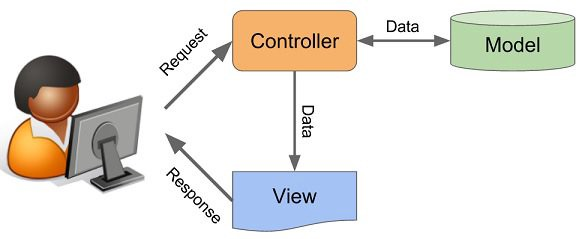
\includegraphics[width=16cm]{figuras/mvc}
  }{
    \Fonte{\citeonline{MVCIMAGE}.}
  }
\end{figure}

\section{Detalhes}

Para que um software possa ser desenvolvido com qualidade de código afim de garantir sua manutenibilidade, extensibilidade e testabilidade é necessário, muitas vezes, a construção de entidades que abstraiam conceitos do domínio do problema. Nesse sentido, esse projeto usou os conceitos descritos no SOLID para alcançar esse objetivo.

Nesse sentido, buscando atender as diretivas descritas pelo SOLID, afim de garantir a qualidade e longevidade do software, o seguinte modelo conceitual simplificado, de acordo com a UML foi gerado:


\begin{alineascomponto}
  \item \textbf{Jogador:} Define a pessoa que entrou no jogo, independente de estar registrado ou não
  \item \textbf{Desafio:} Define o desafio de memória, que possui níveis de dificuldade e temas de cartas para serem memorizadas dentro das regras do jogo da memória.  
  \item \textbf{Tema de Cartas:} Define um conjunto de cartas para serem memorizadas, conceitualmente um tema de cartas lida com cartas que representam um mesmo contexto do mundo real.
  \item \textbf{Mesa de jogo:} Define um lugar onde 1 ou mais jogadores se reúnem para disputar um desafio do jogo da memória 
  \item \textbf{Cartas:}  Define os itens a serem memorizados, possuindo uma imagem associada, e um som. As cartas farão parte de um tema de cartas, e através dele sera, usadas em um desafio. 
\end{alineascomponto}


A figura \ref{fig:modeloconceitual} explicita os conceitos, seus atributos e suas relações


\begin{figure}[h!]
  \centering
  \Caption{\label{fig:modeloconceitual} Modelo Conceitual}
  \UFCfig{}{
    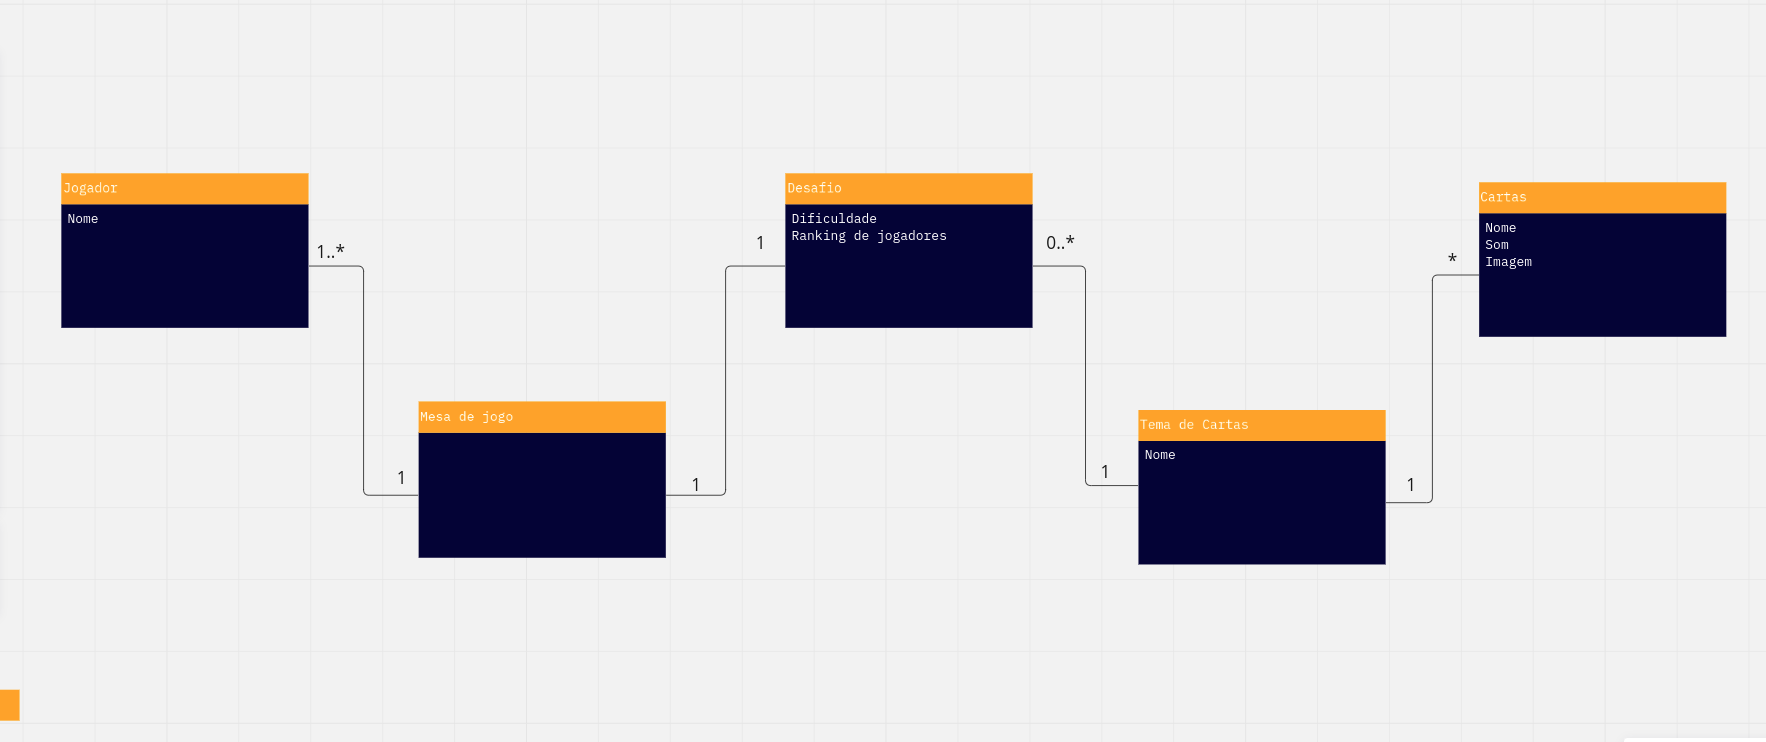
\includegraphics[width=16cm]{figuras/diagrama-conceitual.png}
  }{
    \Fonte{Criada pelo autor.}
  }
\end{figure}






